\documentclass[12pt]{article}

\usepackage[hungarian]{babel}
\usepackage{t1enc}
\usepackage[utf8]{inputenc}
\usepackage[margin=2.5cm]{geometry}
\usepackage{setspace}
\usepackage{graphicx}
\usepackage{float}
\usepackage{hanging}
\PassOptionsToPackage{hyphens}{url}\usepackage{hyperref}

\hypersetup{
    colorlinks,
    citecolor=black,
    filecolor=black,
    linkcolor=black,
    urlcolor=blue
}

\graphicspath{ {./figs/} }
\setlength{\belowcaptionskip}{5pt plus 3pt minus 2pt}

\setstretch{1.5}

\begin{document}

\begin{titlepage}
	\begin{center}
		\vspace*{5cm}
		
		\Huge
		\textbf{Kockázatmodellezés és -előrejelzés}
		
		\vspace{2cm}
		
		\LARGE
		Salamon András, Szilágyi Gergő
		
		\vfill
		
		\Large
		Hitelek és kockázatok makro és mikro szinten \\

        \vspace{1cm}
        
        2023. tavaszi félév
            
    \end{center}
\end{titlepage}

\newgeometry{margin=2.5cm}

\tableofcontents

\clearpage

\listoffigures

\clearpage

\section{Historikus VaR}



\section{Szimulált VaR}



\section{EWMA}

Az EWMA (Exponentially Weighted Moving Average) segítségével szimulálható a pénzpiacokon megfigyelhető volatilitásklasztereződés. Eszerint azokat a napokat volatilisebb napok követik, amelyeken jobban ingadozik az árfolyam, valamint ez fordítva is igaz, a nyugodtabb napokat nyugodtabb napok követik. Az EWMA-ban az előző időszaki loghozamok négyzetét exponenciálisan csökkenő súlyokkal súlyozzuk. Az, hogy mennyire gyors az exponenciális csökkenés, a decay faktor értéke határozza meg. A súlyokat egyre normálva nagyobb decay faktor mellett kisebb súlyokat kapunk, azonban a súlyok lassabban csökkennek.

\begin{figure}[H]
	\centering
	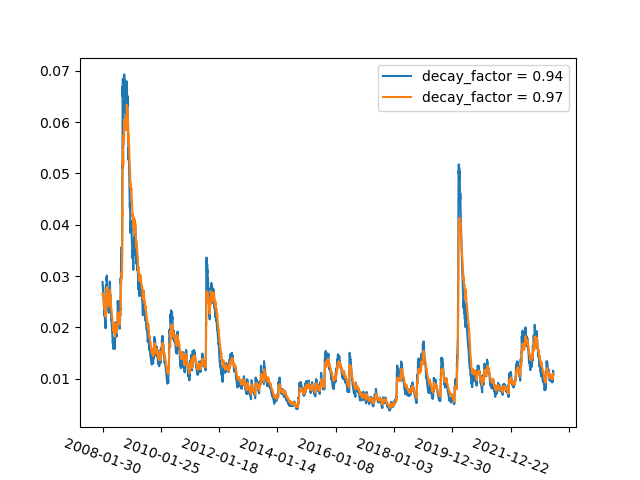
\includegraphics[scale=0.8]{ewma}
	\caption{EWMA a MOO idősoros adatokon a két decay faktor mellett}
\end{figure}

Ahogy az ábrán látható, nagyobb decay faktor mellett nagyobb az előrejelzett volatilitás, azonban ebben az esetben a volatilitások jobban klasztereződnek, mivel nem olyan nagyok a kilengések, mint kisebb decay faktor mellett.


\section{Machine Learning}



\end{document}














